\documentclass[10pt]{article}
\bibliographystyle{IEEEtran}
\usepackage[utf8]{inputenc}
\usepackage[letterpaper, left=1.25in, right=1.25in, bottom=1in, top=1in]{geometry}
\usepackage{amsmath}
\usepackage{pgfplotstable}
\usepackage{booktabs}
\usepackage{multicol}
\usepackage{fancyhdr}
\usepackage{dirtree}
\usepackage{listings}
\usepackage{hyperref}
\usepackage{tensor}
\usepackage{listings}
\usepackage{color}

\definecolor{mygreen}{RGB}{28,172,0}
\definecolor{mylilas}{RGB}{170,55,241}
\renewcommand{\listtablename}{Matlab Files} 

\lstloadlanguages{Matlab}%
\lstset{language=Matlab,%
    %basicstyle=\color{red},
    basicstyle=\fontfamily{pcr}\selectfont,
    breaklines=true,%
    morekeywords={matlab2tikz},
    keywordstyle=\color{blue},%
    morekeywords=[2]{1}, keywordstyle=[2]{\color{black}},
    identifierstyle=\color{black},%
    stringstyle=\color{mylilas},
    commentstyle=\color{mygreen},%
    showstringspaces=false,%without this there will be a symbol in the places where there is a space
    numbers=left,%
    numberstyle={\tiny \color{black}},% size of the numbers
    numbersep=10pt, % this defines how far the numbers are from the text
    emph=[1]{for,end,break},emphstyle=[1]\color{red}, %some words to emphasise
    %emph=[2]{word1,word2}, emphstyle=[2]{style},    
}

\usepackage{listings}

%\definecolor{mygreen}{RGB}{28,172,0}
%\definecolor{mylilas}{RGB}{170,55,241}
\renewcommand{\listtablename}{C} 

\lstloadlanguages{C}%
\lstset{language=C,%
    %basicstyle=\color{red},
    basicstyle=\fontfamily{lmtt}\selectfont,
    breaklines=true,%
    showstringspaces=false,%without this there will be a symbol in the places where there is a space
    numbers=left,%
    numberstyle={\color{black}},% size of the numbers
    numbersep=10pt, % this defines how far the numbers are from the text
}


\newcommand{\PP}{\par\hspace{1cm}}
\newcommand{\uu}{\underline}
\newcommand{\blockstart}{\vspace{1cm}\begin{minipage}{\linewidth}}
\newcommand{\blockstop}{\end{minipage}}

\pgfplotsset{compat=1.14}
\begin{document}
\blockstart
\section*{Overview}
\PP This project contains MATLAB files created to visualize and verify quaternion calculations, specifically those employed in Madgwick 2010 \cite{Madgwick10}. This document was made to show which code matches with which equations in Madgwick 2010 \cite{Madgwick10} and to discuss some results. To quickly view a rotation of a vector by defined by a given quaternion, run \textbf{driver.m}.
\blockstop

\blockstart
\section*{Selected Code}

\vspace{1cm}
\begin{align}
\boldsymbol{a} \otimes \boldsymbol{b} &= \begin{bmatrix} a_1 & a_2 & a_3 & a_4 \end{bmatrix} \otimes \begin{bmatrix} b_1 & b_2 & b_3 & b_4 \end{bmatrix} \notag \\
&= \begin{bmatrix} 
a_1 b_1 - a_2 b_2 - a_3 b_3 - a_4 b_4 \\ 
a_1 b_2 + a_2 b_1 + a_3 b_4 - a_4 b_3 \\ 
a_1 b_3 - a_2 b_4 + a_3 b_1 + a_4 b_2 \\
a_1 b_4 + a_2 b_3 - a_3 b_2 + a_4 b_1 \end{bmatrix}^T \tag{4, Madgwick}
\end{align}

\subsubsection*{quatMult.m}
%\lstinputlisting[language=Matlab,firstnumber=6,firstline=6,lastline=6]{quatMult.m}
\lstinputlisting[language=Matlab,firstnumber=28,firstline=28,lastline=37]{quatMult.m}
\blockstop

\blockstart
\vspace{1cm}
\begin{align}
\tensor[^B]{\boldsymbol{\upsilon}}{} = \tensor*[^{A}_B]{\boldsymbol{\hat{q}}}{} \otimes \tensor[^A]{\boldsymbol{\upsilon}}{} \otimes \tensor*[^{A}_B]{\boldsymbol{\hat{q}}}{^*} \tag{5, Madgwick}
\end{align}

\subsubsection*{quatRotateDup.m}
\lstinputlisting[language=Matlab,firstnumber=9,firstline=9,lastline=13]{quatRotateDup.m}
\blockstop

\blockstart
\section*{Example}
\PP The below figure demonstrates the result of \textbf{driver.m} for a $\pi/4$ angle rotation about the z axis. The initial vector [1 0 0], a unit vector in the x axis, was hardcoded in \textbf{quatTest.m}.

\begin{center}
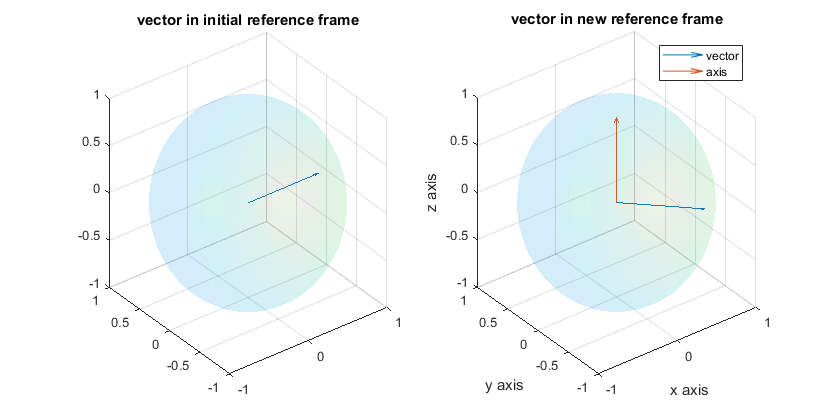
\includegraphics[width = 16cm]{./snap1.png}
\end{center}
\blockstop


\blockstart
\section*{Directory Tree}
\begin{flushleft}
\dirtree{%
.1 {./}.
.2 {README.md}.
.2 {driver.m}.
.2 {quatRotateDup.m}.
.2 {quatMult.m}.
.2 {quatTest.m}.
}
\end{flushleft}
\blockstop

\newpage
\section*{README.md}
\lstinputlisting[language=C]{README.md}

\blockstart\bibliography{references}\blockstop

\end{document}
